\documentclass[preprint,12pt]{elsarticle}

\usepackage{amsmath,amssymb,amsthm,booktabs,graphicx}
\usepackage{microtype}
\usepackage{hyperref}
\hypersetup{hidelinks}
\usepackage{siunitx}
\usepackage{enumitem}
\usepackage{placeins}

\journal{Journal of Computational and Applied Mathematics}

\newtheorem{theorem}{Theorem}
\newtheorem{proposition}[theorem]{Proposition}
\newtheorem{lemma}[theorem]{Lemma}
\newtheorem{corollary}[theorem]{Corollary}
\theoremstyle{remark}
\newtheorem{remark}[theorem]{Remark}

\begin{document}

\begin{frontmatter}

\title{From Structural Minimax to Gauss--Legendre:
A Positive Moment-Constrained Stieltjes Quadrature Hierarchy}

\author[inst1]{Tran Minh Duc\corref{cor1}}
\cortext[cor1]{Corresponding author}
\ead{ductranminh2107@gmail.com}

\affiliation[inst1]{
  organization={FPT University},
  addressline={Lot E2a-7, D1 Street, Saigon Hi-Tech Park},
  city={Ho Chi Minh City},
  country={Vietnam}
}

\begin{abstract}
We study positive symmetric quadrature rules for a
centered Lorentzian/Stieltjes family under a variable number of moment
conditions. With \(n\) positive node pairs and moment depth \(k\), the
full feasible range is \(0\leq k\leq 2n\). The admissible set is a smooth
manifold of dimension \(2n-k\); moment depths above \(2n\) are impossible,
and the endpoint \(k=2n\) is exactly the classical \(2n\)-point
Gauss--Legendre rule. For \(k<2n\), shared Laurent coefficients reduce
the degree of the difference numerator to \(2n-k-1\), giving a
\(2n-k+1\)-point alternation certificate for minimaxity within the
stated class. Complete high-precision hierarchies for \(n=2,3,4\)
quantify the transition from structural minimax to Gaussian exactness.
For a smooth residual with Chebyshev coefficients
\(|a_j|\leq C\rho^{-j}\), we derive the exact worst-case error
\(C G_k(\rho)\). Combining this quantity with the structural error
\(S_k\) gives the exact model-aware risk
\(G_k(\rho)+\tau S_k\). Conservative numerical enclosures assign a
unique rule on 97.9067\% of the tested parameter domain.
Seventy-two multi-start reconstructions recover the upper-half rules,
and a shifted-Lorentzian stress test supports local, rather than
universal, robustness.
\end{abstract}

\begin{keyword}
numerical quadrature \sep Stieltjes functions \sep rational minimax
approximation \sep moment constraints \sep Gauss--Legendre quadrature
\sep validated numerics
\end{keyword}

\end{frontmatter}

\section{Introduction}

Gaussian quadrature allocates a fixed node budget to polynomial
exactness. This is a powerful default for smooth integrands, but it need
not be the most effective design when the dominant difficulty is a
known nearby pole. Rationally exact quadrature incorporates prescribed
singular structure \cite{gautschi1993}, generalized Gaussian rules extend
exactness to non-polynomial function systems \cite{huybrechs2017}, and
optimization-based constructions provide flexible ways to determine
nodes and weights \cite{keshavarzzadeh2018,glaubitz2020}. Rational
approximation of Markov and Stieltjes functions supplies closely related
structural theory \cite{beckermann2021}.

The present problem lies between two extremes. At one end, an
unconstrained rule can devote all of its degrees of freedom to a
near-singular structural family. At the other, the Gauss--Legendre rule
devotes the full budget to polynomial exactness. The central question is
whether these endpoints belong to a single controlled hierarchy and,
if so, how the intermediate rule should be selected when the integrand
also contains an uncertain smooth background.

We answer this question within the class of positive symmetric
Stieltjes-response rules. The paper does not claim novelty for
positivity, moment matching, minimax approximation, or Gaussian
quadrature separately. Its contribution is the combined framework:
\begin{enumerate}[label=(\roman*)]
\item the full feasible moment range \(0\leq k\leq2n\), the dimension
law \(\dim\mathcal A_{n,k}=2n-k\), impossibility beyond \(2n\), and
identification of the endpoint with Gauss--Legendre;
\item a degree-reduction argument and a class-specific alternation
certificate for every nonzero-dimensional level;
\item complete numerical hierarchies for \(n=2,3,4\), including the
previously missing upper-half rules;
\item an exact coefficient-space risk and full-hierarchy rule selector;
\item conservative numerical validation of the rounded rules, a
shifted-family stress test, and independent multi-start reconstruction.
\end{enumerate}

These claims are restricted to the stated symmetric positive class.
They do not imply universal superiority over Gaussian, adaptive, or
problem-specific quadrature outside the modeled setting.

\section{Problem formulation}

Let
\[
I[f]=\int_{-1}^{1} f(x)\,dx,
\qquad
L_b(x)=\frac{1}{x^2+b^2},
\qquad
b\in B=[0.08,0.12].
\]
With \(s=b^2\) and \(y=x^2\),
\[
F(s)=I[L_{\sqrt{s}}]
=\int_0^1\frac{y^{-1/2}}{s+y}\,dy
=\frac{2}{\sqrt{s}}\arctan\frac{1}{\sqrt{s}}.
\]
A symmetric \(n\)-pair rule has the form
\[
Q[f]=\sum_{j=1}^{n}w_j\{f(-x_j)+f(x_j)\},
\qquad
0<x_1<\cdots<x_n<1,\quad w_j>0.
\]
Writing \(y_j=x_j^2\), the response on the structural family is the
positive Stieltjes rational function
\[
r_Q(s)=Q[L_{\sqrt{s}}]
=2\sum_{j=1}^{n}\frac{w_j}{s+y_j}.
\]

For an integer \(k\geq0\), define the moment-constrained class
\[
\mathcal A_{n,k}
=
\left\{
Q:
\sum_{j=1}^{n}w_jy_j^\ell=\frac{1}{2\ell+1},
\quad \ell=0,\ldots,k-1
\right\}.
\]
For \(k=0\), no moment condition is imposed.

\begin{lemma}[Equivalent interpretations of the constraints]
For \(k\geq1\), the following conditions are equivalent:
\begin{enumerate}[label=(\alph*)]
\item \(Q\in\mathcal A_{n,k}\);
\item \(Q\) is exact for every polynomial of degree at most \(2k-1\);
\item \(r_Q(s)-F(s)=O(s^{-k-1})\) as \(s\to\infty\).
\end{enumerate}
\end{lemma}

\begin{proof}
Symmetry gives exactness for odd polynomials. For even monomials,
\[
Q[x^{2\ell}]=2\sum_{j=1}^{n}w_jy_j^\ell,
\qquad
I[x^{2\ell}]=\frac{2}{2\ell+1},
\]
which proves the equivalence of (a) and (b). The expansion
\[
\frac{1}{s+y}
=
\sum_{\ell=0}^{m-1}(-1)^\ell y^\ell s^{-\ell-1}
+O(s^{-m-1})
\]
is uniform for \(y\in[0,1]\). Integrating it against
\(y^{-1/2}\,dy\) and applying it to the discrete measure
\(2\sum_jw_j\delta_{y_j}\) proves the equivalence with (c).
\end{proof}

\section{The full feasible hierarchy}

Let
\[
\mathcal P_n
=
\{(y,w):
0<y_1<\cdots<y_n<1,\ w_j>0\}
\subset\mathbb R^{2n},
\]
and define the moment map
\[
M_k(y,w)
=
\left(
\sum_{j=1}^{n}w_jy_j^\ell
\right)_{\ell=0}^{k-1}.
\]

\begin{theorem}[Feasible range, dimension, and Gaussian endpoint]
Within the positive ordered class:
\begin{enumerate}[label=(\roman*)]
\item \(\mathcal A_{n,k}\) is nonempty for every \(0\leq k\leq2n\);
\item for \(0\leq k\leq2n\), it is a smooth manifold of dimension
\[
\dim\mathcal A_{n,k}=2n-k;
\]
\item \(\mathcal A_{n,k}\) is empty for \(k>2n\);
\item \(\mathcal A_{n,2n}\) consists of the positive half of the
classical \(2n\)-point Gauss--Legendre rule.
\end{enumerate}
\end{theorem}

\begin{proof}
Nonemptiness follows because the \(2n\)-point Gauss--Legendre rule
satisfies all moment conditions through \(k=2n\), and hence every
prefix.

To prove the rank statement, suppose a linear combination of the rows
of \(DM_k\) vanishes and define
\[
p(y)=\sum_{\ell=0}^{k-1}c_\ell y^\ell.
\]
The columns obtained by differentiating with respect to \(w_j\) give
\(p(y_j)=0\), while the columns obtained by differentiating with respect
to \(y_j\) give \(w_jp'(y_j)=0\). Positivity implies
\(p'(y_j)=0\). Thus every \(y_j\) is a double root. For
\(k\leq2n\), however, \(\deg p\leq2n-1\), so \(p\equiv0\).
Therefore \(DM_k\) has full row rank \(k\), and the implicit-function
theorem gives dimension \(2n-k\).

For impossibility, suppose moments through index \(2n\) were matched.
The polynomial
\[
g(y)=\prod_{j=1}^{n}(y-y_j)^2
\]
has degree \(2n\), is nonnegative, and is not identically zero. The
discrete transformed rule gives \(2\sum_jw_jg(y_j)=0\), whereas
\[
\int_0^1g(y)y^{-1/2}\,dy>0,
\]
a contradiction.

At \(k=2n\), the transformed \(n\)-node rule is exact through degree
\(2n-1\) for the measure \(y^{-1/2}\,dy\). It is therefore its Gaussian
quadrature rule. Under \(y=x^2\), the symmetric rule is exact through
degree \(4n-1\), and hence is the \(2n\)-point Gauss--Legendre rule.
\end{proof}

\begin{remark}
The previously studied range \(0\leq k\leq n\) is the lower half of the
feasible hierarchy. It retains at least \(n\) structural design degrees
of freedom. It is a meaningful high-structural-accuracy regime, but it
is not the maximal feasible range.
\end{remark}

\section{Minimax characterization}

Write two structural responses as \(r_i=p_i/q_i\), where \(q_i\) is
monic of degree \(n\).

\begin{proposition}[Difference-numerator degree]
If \(r_1,r_2\in\mathcal A_{n,k}\) and \(0\leq k\leq2n\), then
\[
r_1-r_2=\frac{H}{q_1q_2},
\qquad
\deg H\leq2n-k-1,
\]
unless the two responses are identical.
\end{proposition}

\begin{proof}
The generic numerator \(p_1q_2-p_2q_1\) has degree at most \(2n-1\).
The shared Laurent coefficients imply
\(r_1-r_2=O(s^{-k-1})\). Since \(q_1q_2\) is monic of degree \(2n\),
the stated degree bound follows.
\end{proof}

Define the relative structural error
\[
\varepsilon_Q(s)=\frac{r_Q(s)}{F(s)}-1.
\]

\begin{theorem}[Alternation certificate]
Let \(0\leq k<2n\). Suppose \(Q^\star\in\mathcal A_{n,k}\) has
\(2n-k+1\) ordered points on the design interval at which
\(\varepsilon_{Q^\star}\) has equal magnitude and alternating sign, and
this magnitude equals its uniform norm. Then no rule in
\(\mathcal A_{n,k}\) has strictly smaller uniform relative error.
\end{theorem}

\begin{proof}
A strictly better competitor would make
\(\varepsilon_{Q^\star}-\varepsilon_Q\) alternate sign at the
\(2n-k+1\) points, forcing at least \(2n-k\) distinct zeros. Since
\(F(s)>0\), these are zeros of \(r_{Q^\star}-r_Q\), contradicting the
degree bound \(2n-k-1\), unless the responses are identical.
\end{proof}

\begin{remark}
The theorem proves minimaxity within the stated class, not global
uniqueness of the nonlinear parameterization. The zero-dimensional
endpoint \(k=2n\) is determined by its moments and does not require a
nontrivial alternation argument.
\end{remark}

\section{Numerical construction of the complete hierarchy}

The constrained minimax equations combine the \(k\) moment conditions,
equal-magnitude alternating errors, and stationarity at internal
extrema. Lower-half rules were constructed in high precision. The
missing upper-half problems were solved by continuation toward the
Gaussian endpoint and refined through the equioscillation equations.
All published rules have ordered nodes and positive weights.

\begin{table}[ht]
\centering
\caption{Complete \(n=4\) hierarchy. The endpoint \(k=8\) is
zero-dimensional; therefore the alternation-certificate column is not
applicable.}
\label{tab:full-hierarchy}
\small
\begin{tabular}{cccccc}
\toprule
\(k\) & Dimension & Exactness & Cert. points &
Worst relative error & Min. \(w_j\)\\
\midrule
0 & 8 & -- & 9 & 1.490623e-10 & 0.039147 \\
1 & 7 & 1 & 8 & 2.460626e-09 & 0.044528 \\
2 & 6 & 3 & 7 & 4.048641e-08 & 0.051670 \\
3 & 5 & 5 & 6 & 6.653546e-07 & 0.061646 \\
4 & 4 & 7 & 5 & 1.092819e-05 & 0.076595 \\
5 & 3 & 9 & 4 & 1.794333e-04 & 0.101407 \\
6 & 2 & 11 & 3 & 2.943219e-03 & 0.149011 \\
7 & 1 & 13 & 2 & 4.597982e-02 & 0.126194 \\
8 & 0 & 15 & -- & 4.300499e-01 & 0.101229 \\
\bottomrule
\end{tabular}
\end{table}

\begin{figure}[ht]
\centering
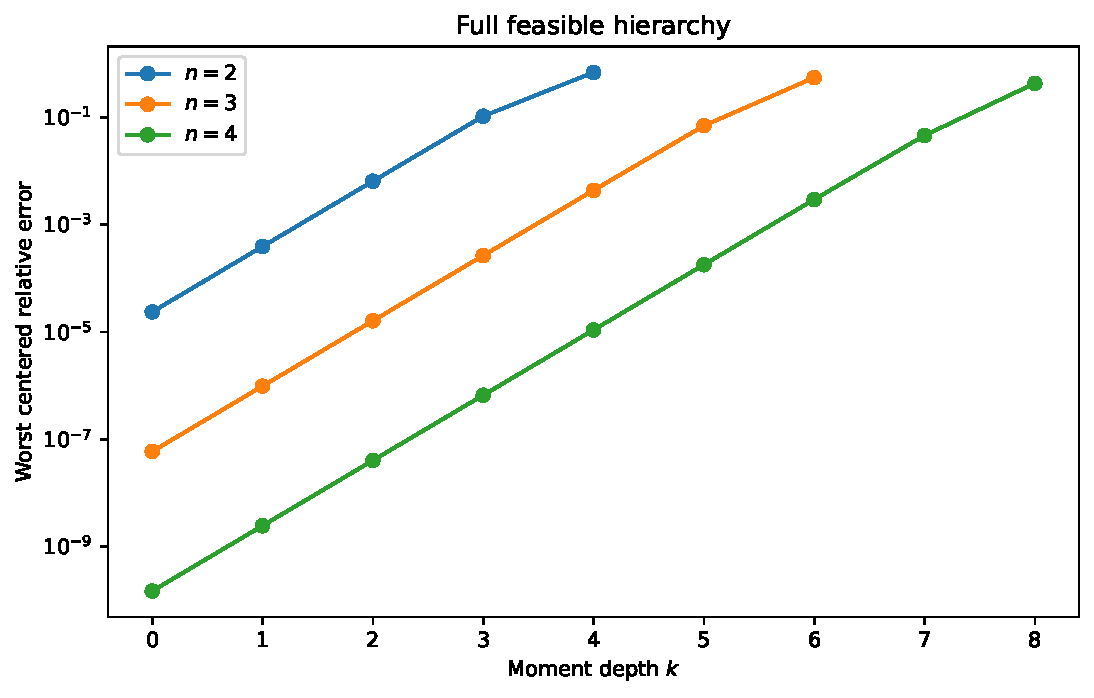
\includegraphics[width=0.84\linewidth]{figures/figure1_full_hierarchy.pdf}
\caption{Worst centered relative error for the full feasible
hierarchies \(0\leq k\leq2n\), \(n=2,3,4\). The final point of each
curve is the corresponding Gauss--Legendre rule.}
\label{fig:full-hierarchy}
\end{figure}

For \(n=4\), the error grows from \(1.49\times10^{-10}\) at \(k=0\) to
\(4.30\times10^{-1}\) at the Gauss endpoint. The upper-half values
\(k=5,6,7\) continue the approximately constant finite-range price per
additional moment before the error enters an order-one regime. This
pattern is empirical and is not claimed as an asymptotic theorem.

\begin{figure}[ht]
\centering
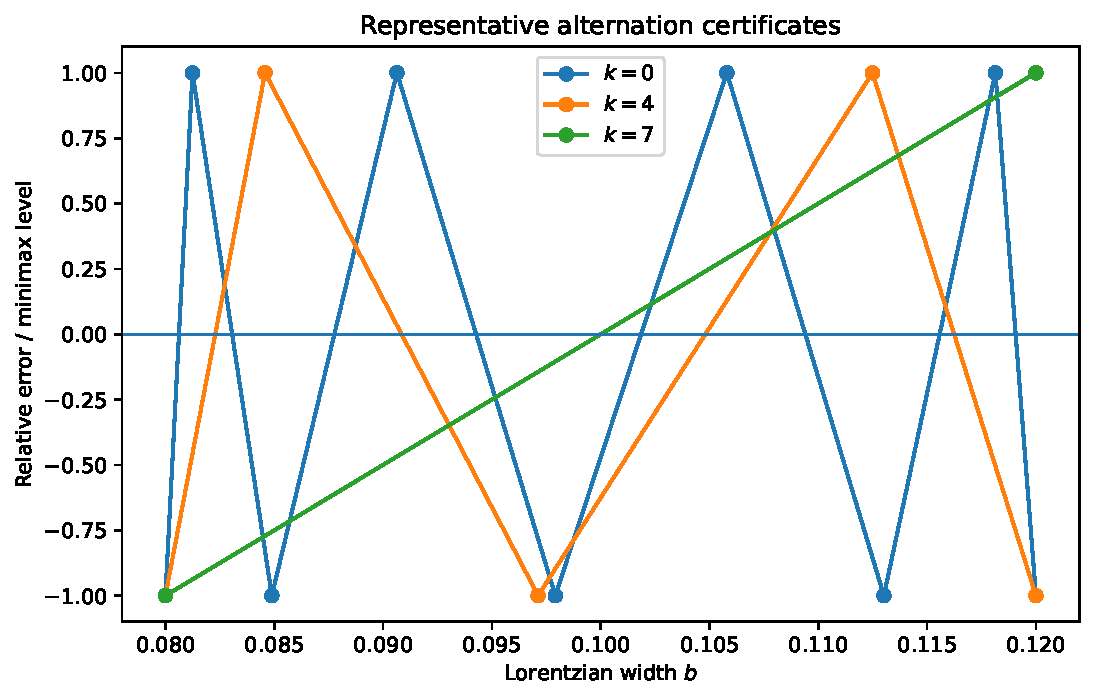
\includegraphics[width=0.82\linewidth]{figures/figure2_alternation.pdf}
\caption{Representative normalized alternation patterns from the lower
endpoint (\(k=0\)), midpoint (\(k=4\)), and upper half (\(k=7\)) of the
\(n=4\) hierarchy.}
\label{fig:alternation}
\end{figure}

\FloatBarrier

\section{Exact coefficient-space rule selection}

Let the uncertain smooth residual have a Chebyshev expansion
\[
h(x)=\sum_{j=0}^{\infty}a_jT_j(x),
\qquad
|a_j|\leq C\rho^{-j},
\quad \rho>1.
\]
For a fixed rule, define
\[
\Delta_j(Q)=I[T_j]-Q[T_j].
\]

\begin{theorem}[Exact coefficient-box norm]
For every fixed bounded quadrature rule,
\[
\sup_h |I[h]-Q[h]|
=
C G_Q(\rho),
\qquad
G_Q(\rho)
=
\sum_{j=0}^{\infty}\rho^{-j}|\Delta_j(Q)|.
\]
\end{theorem}

\begin{proof}
Uniform convergence allows termwise application of \(I-Q\). The
triangle inequality gives the upper bound, and it is attained by the
sign-aligned coefficients
\[
a_j=C\rho^{-j}\operatorname{sign}\Delta_j(Q).
\]
\end{proof}

For the mixed class
\[
f(x)=h(x)+cL_b(x),
\qquad
|c|\leq c_{\max},
\]
define
\[
S_Q=\max_{b\in B}|I[L_b]-Q[L_b]|.
\]

\begin{theorem}[Exact mixed-class risk]
For every fixed rule,
\[
\sup_f |I[f]-Q[f]|
=
C G_Q(\rho)+c_{\max}S_Q.
\]
\end{theorem}

The two signs can be chosen independently. For \(C>0\), define
\(\tau=c_{\max}/C\). The model-aware rule is therefore
\[
k^\star(\rho,\tau)
\in
\arg\min_{0\leq k\leq2n}
\left[G_k(\rho)+\tau S_k\right].
\]

\begin{table}[ht]
\centering
\caption{Full \(n=4\) structural and smooth-risk trade-off at
\(\rho=1.5\).}
\label{tab:risk-components}
\small
\begin{tabular}{ccc}
\toprule
\(k\) & Structural upper enclosure \(S_k\) & \(G_k(1.5)\)\\
\midrule
0 & 5.55627e-09 & 9.11242e-01 \\
1 & 9.17189e-08 & 3.95465e-01 \\
2 & 1.50911e-06 & 2.04657e-01 \\
3 & 2.48007e-05 & 9.59856e-02 \\
4 & 4.07341e-04 & 4.49242e-02 \\
5 & 6.68824e-03 & 2.14018e-02 \\
6 & 1.09706e-01 & 1.17665e-02 \\
7 & 1.71386e+00 & 6.62192e-03 \\
8 & 1.60298e+01 & 3.42291e-03 \\
\bottomrule
\end{tabular}
\end{table}

\begin{figure}[ht]
\centering
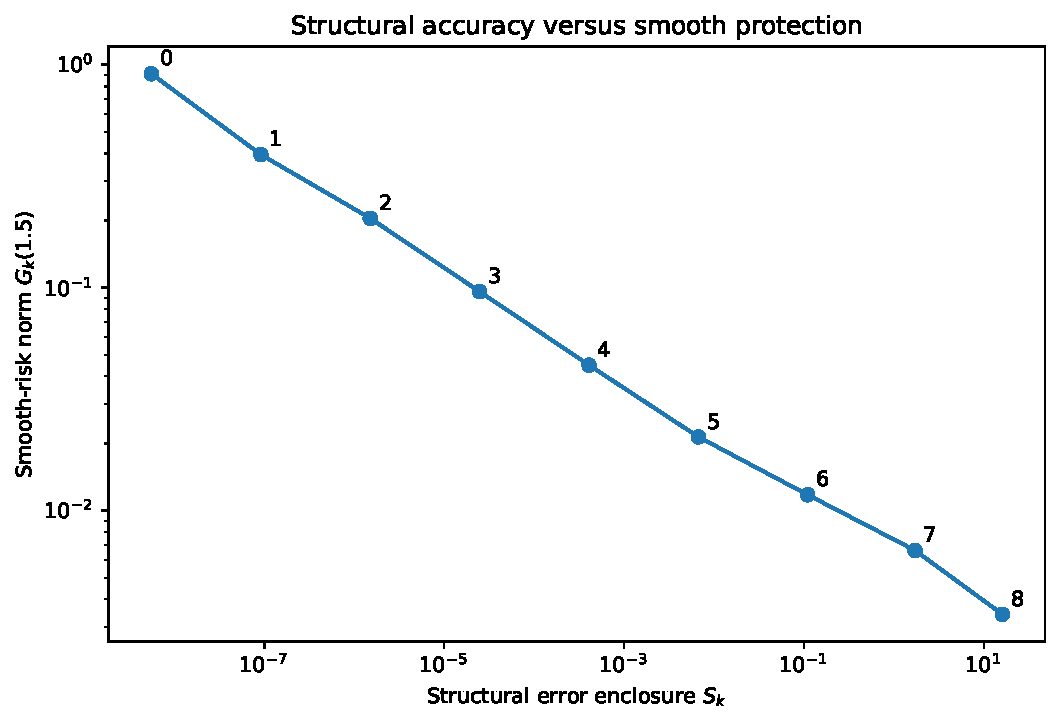
\includegraphics[width=0.78\linewidth]{figures/figure3_risk_tradeoff.pdf}
\caption{Each added moment decreases the smooth-risk norm but increases
the Lorentzian structural error. Labels indicate the moment depth
\(k\).}
\label{fig:risk-tradeoff}
\end{figure}

\section{Validated partition for the rounded rules}

The exact hierarchy theory concerns ideal moment-constrained rules.
Published decimal nodes and weights have small rounding defects.
The coefficient-box risk remains exact for each fixed rounded operator,
but a nominal moment label alone does not transfer exact symbolic
properties.

We therefore re-evaluated all nine rounded \(n=4\) rules. The expected
alternation counts were recovered for \(k=0,\ldots,7\). Structural
errors were enclosed by a dense partition and inflated local derivative
bounds. Chebyshev defects were evaluated through degree 500, and the
remaining tail was bounded geometrically. A parameter cell was assigned
a rule only when its risk upper bound was below the lower bounds of all
competitors throughout the cell.

Adaptive refinement assigned a unique winner on
\[
97.9067\%
\]
of
\[
(\rho,\log_{10}\tau)
\in[1.05,5]\times[-12,12].
\]
The unresolved area, \( 2.0933\% \), is concentrated near
transition curves.

\begin{table}[ht]
\centering
\caption{Fraction of the certified parameter area assigned to each
moment depth.}
\label{tab:selection-fractions}
\small
\begin{tabular}{cc}
\toprule
\(k\) & Certified-area fraction\\
\midrule
0 & 22.279\% \\
1 & 9.216\% \\
2 & 8.299\% \\
3 & 8.463\% \\
4 & 8.478\% \\
5 & 8.460\% \\
6 & 8.117\% \\
7 & 6.934\% \\
8 & 19.753\% \\
\bottomrule
\end{tabular}
\end{table}

\begin{figure}[ht]
\centering
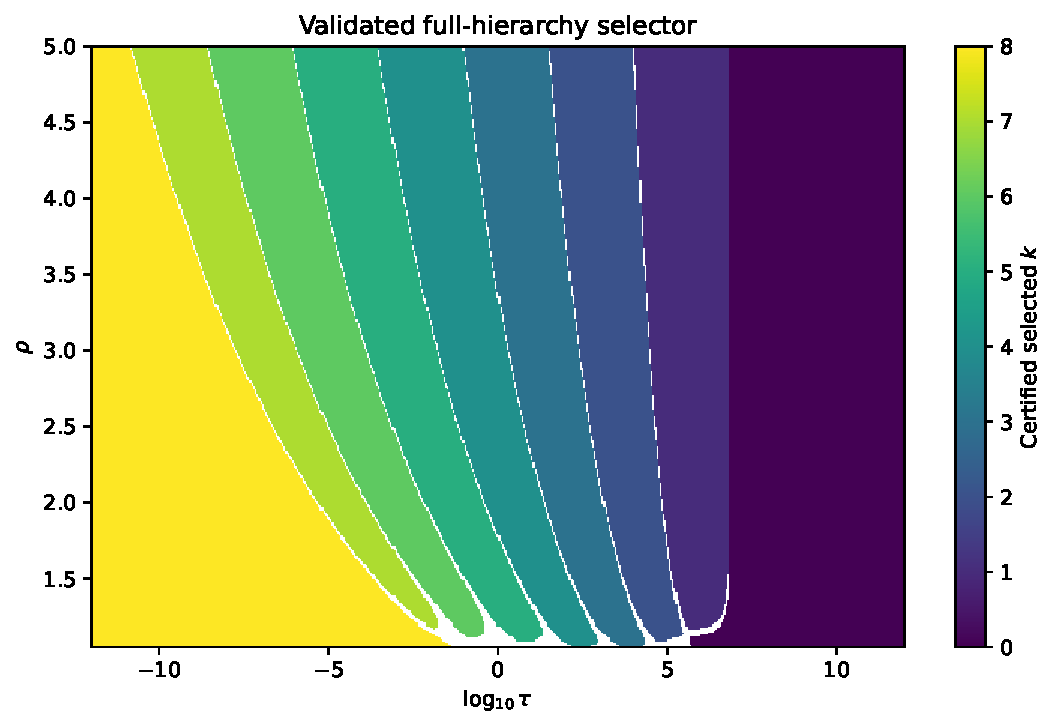
\includegraphics[width=0.84\linewidth]{figures/figure4_certified_selector.pdf}
\caption{Validated full-hierarchy selector. Blank regions are not
assigned because the conservative risk enclosures overlap.}
\label{fig:selector}
\end{figure}

This validation is numerical rather than proof-assistant formal.
The reported coverage depends on the stated enclosures and refinement
depth.

\FloatBarrier

\section{External validity and reconstruction}

\subsection{Small pole-location mismatch}

Without retraining, the centered rules were tested on
\[
L_{a,b}(x)=\frac{1}{(x-a)^2+b^2},
\qquad
|a|\leq0.03,
\quad
0.08\leq b\leq0.12.
\]

\begin{table}[ht]
\centering
\caption{Worst relative errors on the shifted-Lorentzian stress-test
box.}
\label{tab:shifted}
\small
\begin{tabular}{lcccc}
\toprule
Method & Evaluations & Worst error & Worst \(|a|\) & Worst \(b\)\\
\midrule
PMC--k0 & 8 & 4.522336e-06 & 0.0300 & 0.0800 \\
PMC--k4 & 8 & 1.025564e-03 & 0.0300 & 0.0845 \\
Composite--Simpson--9 & 9 & 7.426762e-02 & 0.0300 & 0.1200 \\
Gauss--Legendre--8 & 8 & 4.300499e-01 & 0.0000 & 0.0800 \\
\bottomrule
\end{tabular}
\end{table}

\begin{figure}[ht]
\centering
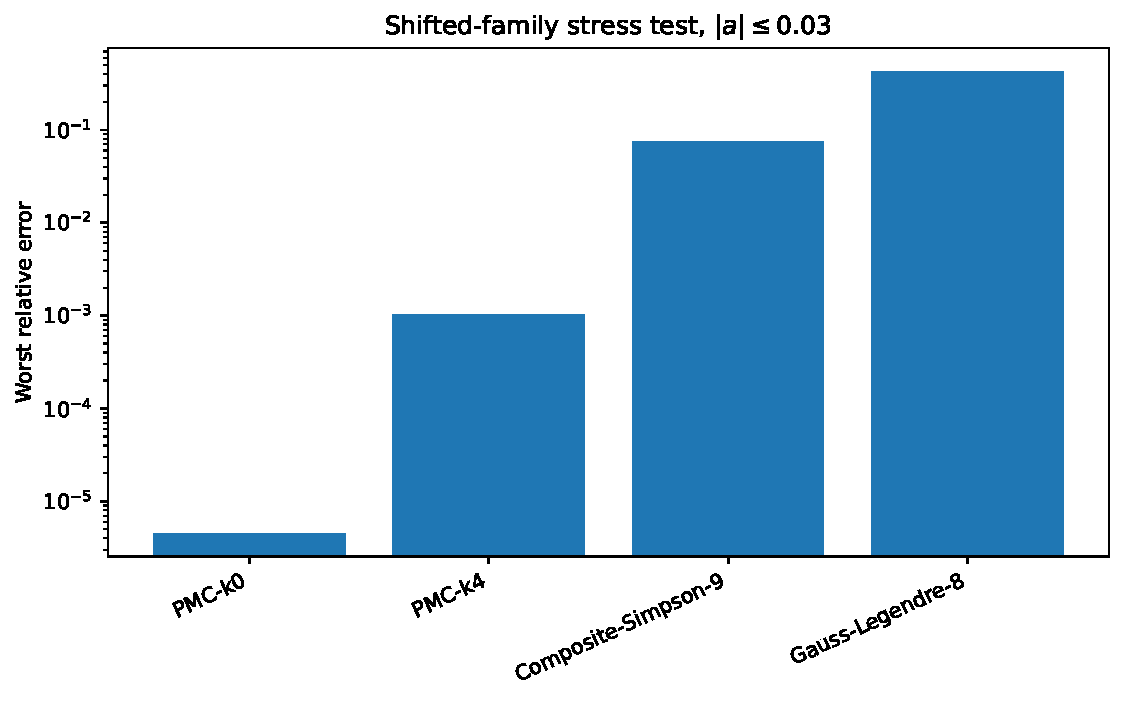
\includegraphics[width=0.82\linewidth]{figures/figure5_shifted_stress.pdf}
\caption{Stress test under small pole-location mismatch. The comparison
supports local structural robustness, not shifted-family minimaxity or
universal superiority.}
\label{fig:shifted}
\end{figure}

The \(k=0\) rule has worst relative error
\(4.52\times10^{-6}\), whereas the Gauss endpoint has worst error
\(4.30\times10^{-1}\) on the same box. The centered error is nevertheless
inflated by more than four orders of magnitude, so the correct
interpretation is local robustness rather than shift invariance.

\subsection{Independent multi-start reconstruction}

The six upper-half problems
\[
(2,3),\ (3,4),\ (3,5),\ (4,5),\ (4,6),\ (4,7)
\]
were reconstructed from twelve perturbed starts each. A run was accepted
only when nodes were ordered, weights were positive, moment residuals
were below \(10^{-10}\), and scaled equioscillation residuals were below
\(10^{-8}\).

\begin{table}[ht]
\centering
\caption{Independent multi-start reconstruction of the upper-half
rules. Error differences are relative to the published minimax level.}
\label{tab:multistart}
\scriptsize
\begin{tabular}{ccccc}
\toprule
\((n,k)\) & Accepted starts & Error difference &
Max. node difference & Max. weight difference\\
\midrule
$(2,3)$ & 12/12 & 2.64e-16 & 5.55e-17 & 5.55e-17 \\
$(3,4)$ & 10/12 & 6.78e-14 & 4.44e-16 & 5.00e-16 \\
$(3,5)$ & 12/12 & 5.31e-14 & 1.29e-14 & 1.32e-14 \\
$(4,5)$ & 8/12 & 2.38e-12 & 4.44e-15 & 4.27e-15 \\
$(4,6)$ & 11/12 & 9.22e-14 & 1.03e-14 & 1.05e-14 \\
$(4,7)$ & 12/12 & 5.11e-13 & 8.95e-14 & 6.43e-14 \\
\bottomrule
\end{tabular}
\end{table}

All accepted solutions in each problem formed a single error-level
cluster. No accepted start found a better rule by more than
\(10^{-6}\) relative, and the maximum best-rule error difference was
\(2.38\times10^{-12}\). This reduces the risk of a local numerical
artifact but is not a proof of global uniqueness or third-party
replication.

\section{Discussion and relation to prior work}

The framework is adjacent to several established directions.
Rationally exact quadrature and generalized Gaussian quadrature use
non-polynomial structural information \cite{gautschi1993,huybrechs2017}.
Positive cubature studies stable positive representations
\cite{glaubitz2020}. Markov-function rational approximation concerns the
same broad Stieltjes geometry \cite{beckermann2021}. Constrained rational
minimax approximation provides especially close methodological context
\cite{zhang2025}. Simultaneous and common-support quadrature constructions
supply further comparisons \cite{vanassche2023,bravo2023}.

The present contribution should therefore not be described as the
invention of structure-aware quadrature, moment matching, positivity, or
minimax approximation. Within the proposed class, the distinctive
combination is the variable-depth path from structural minimax to
Gauss--Legendre, the dimension and feasibility characterization, the
class-specific alternation certificate, and the exact model-aware
selector.

Positivity is retained because it prevents large signed cancellations,
preserves a positive discrete Stieltjes representation, and makes the
Gaussian endpoint part of the same admissible class. Removing positivity
may lower the structural minimax error, but it would define a different
problem with different stability and interpretation.

The selector is useful precisely because no single hierarchy level is
best for the mixed class. Small \(k\) dominates when the structural
component is strong; large \(k\), including the Gaussian endpoint,
occupies substantial parameter regions when the smooth residual
dominates.

\section{Limitations}

The theoretical and numerical study is one-dimensional and symmetric.
The principal structural family is the centered Lorentzian kernel.
The shifted-family experiment is a stress test and is not itself
minimax-optimized or validated by interval arithmetic. Global uniqueness
of the nonlinear minimax parameters is not proved. The full selector
validation leaves approximately 2.0933\% of the domain
unassigned. The empirical near-geometric price per moment is not an
asymptotic theorem. Finally, the novelty positioning still requires
specialist comparison with the closest constrained-rational and
structure-aware quadrature literature.

\section{Conclusion}

The positive moment-constrained Stieltjes rules form a complete feasible
path within the stated class:
\[
k=0
\quad\longrightarrow\quad
k=2n.
\]
The first endpoint is the unconstrained structural minimax rule, while
the second is Gauss--Legendre. Between them, each moment condition
reduces the admissible dimension by one and trades structural accuracy
for smooth polynomial protection. The difference-degree argument gives
a matching alternation count for every nonzero-dimensional level.
An exact coefficient-space risk then turns the hierarchy into a
model-aware selector. Numerical validation, shifted-family testing, and
multi-start reconstruction support the reliability and practical scope
of the computed rules.

\section*{Data and code availability}

The code, published rules, generated data, and reproduction scripts are
available at
\url{https://github.com/TurkeyOp/partial-moment-stieltjes-quadrature}.
The Version 2 upper-half and full-selector materials are included in the
accompanying research archive and should be merged into the public
repository before journal submission.

\section*{Funding}

This research did not receive any specific grant from funding agencies
in the public, commercial, or not-for-profit sectors.

\section*{Declaration of competing interest}

The author declares that he has no known competing financial interests
or personal relationships that could have appeared to influence the
work reported in this paper.

\section*{Declaration of generative AI and AI-assisted technologies in
the manuscript preparation process}

During the preparation of this work, the author used OpenAI ChatGPT to
assist with literature organization, code prototyping, manuscript
structuring, and language revision. The author reviewed and verified
the mathematical derivations, numerical results, references,
interpretations, and final wording and takes full responsibility for
the content of the article.

\begin{thebibliography}{10}
\providecommand{\url}[1]{\texttt{#1}}
\bibitem{gautschi1993} W. Gautschi, Gauss-type quadrature rules for
rational functions, arXiv:math/9307223 (1993).
\bibitem{huybrechs2017} D. Huybrechs, On the computation of Gaussian
quadrature rules for Chebyshev sets of linearly independent functions,
arXiv:1710.11244 (2017).
\bibitem{keshavarzzadeh2018} V. Keshavarzzadeh, R. M. Kirby,
A. Narayan, Generation of nested quadrature rules for generic weight
functions via numerical optimization: Application to sparse grids,
arXiv:1808.03707 (2018).
\bibitem{glaubitz2020} J. Glaubitz, Constructing positive interpolatory
cubature formulas, arXiv:2009.11981 (2020).
\bibitem{beckermann2021} B. Beckermann, J. Bisch, R. Luce, On the
rational approximation of Markov functions, with applications to the
computation of Markov functions of Toeplitz matrices, arXiv:2106.05098
(2021).
\bibitem{trefethen2021} L. N. Trefethen, Exactness of quadrature
formulas, arXiv:2101.09501 (2021).
\bibitem{bravo2023} J. R. Bravo, J. A. Hern\'andez, S. Ares de Parga,
R. Rossi, A subspace-adaptive weights cubature method with application
to local hyperreduction, arXiv:2310.15769 (2023).
\bibitem{vanassche2023} W. Van Assche, A Golub--Welsch version for
simultaneous Gaussian quadrature, arXiv:2309.11864 (2023).
\bibitem{goda2024} T. Goda, Y. Kazashi, K. Tanaka, How sharp are error
bounds? Lower bounds on quadrature worst-case errors for analytic
functions, arXiv:2401.07196 (2024).
\bibitem{zhang2025} L.-H. Zhang, Y.-N. Zhang, b-d-Lawson: a method for
interpolation-constrained rational minimax approximation,
arXiv:2502.10665 (2025).
\end{thebibliography}

\end{document}
